%%%%%%%%%%%%%%%%%%%%%%%%%%%%%%%%%%%%%%%%%%%%%%%%%%%%%%%%%%%%%%%%%%%%%%%%
\section{Introduction}
\label{sec:intro}

%%%%%%%%%%%%%%%%%%%%%%%%%%%%%%%%%%%%%%%%%%%%%%%%%%%%%%%%%%%%%%%%%%%%%%%%
%%%%%%%%%%%%%%%%%%%%%%%%%%%%%%
% moved here from motivation section.
%%%%%%%%%%%%%%%%%%%%%%%%%%%%%%
\begin{figure*}[ht!]
  \centering
    \subfloat[Emulation ]{
      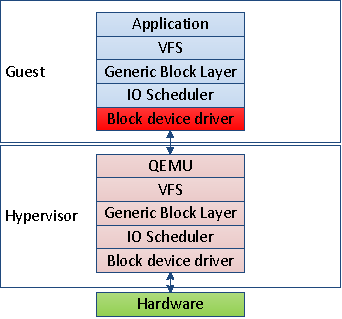
\includegraphics[width=0.3\textwidth]{figs/emulation.pdf}
      \label{fig:storage:emulation}
    }
    \hfill
    \subfloat[virtio]{
      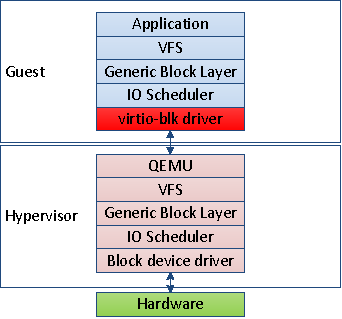
\includegraphics[width=0.3\textwidth]{figs/virtio.pdf}
      \label{fig:storage:virtio}
    }
    \hfill
    \subfloat[Direct-IO]{
      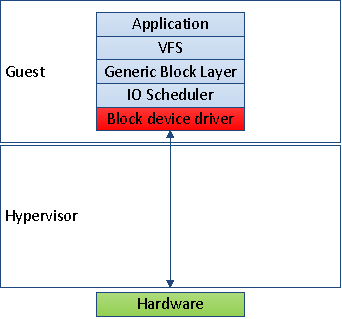
\includegraphics[width=0.3\textwidth]{figs/direct.pdf}
      \label{fig:storage:direct}
    }
    \caption{IO Virtualization techniques.
      \label{fig:storage}}
    
\end{figure*}
%%%%%%%%%%%%%%%%%%%%%%%%%%%%%%

The prevalence of machine consolidation through the use of virtual machines (VMs) necessitates improvements in VM performance. On the architecture side, major processor vendors have introduced virtualization extensions to their instruction set architectures~\cite{popek1974formal,intel,armv8}.
The emergence of high-speed networking interfaces also requires that VMs be granted direct access to  physical devices, thereby eliminating the costly, software-based hypervisor device multiplexing.

Enabling untrusted VMs to directly access physical devices, however, compromises system security.
To overcome the fundamental security issue, the PCIe specification was extended to support self-virtualizing devices through the Single-Root I/O Virtualization (SR-IOV) interface~\cite{pcisigiov}).
This method enables a physical device (\emph{physical function} in SR-IOV parlance) to dynamically create virtual instances (\emph{virtual functions}). Each virtual instance receives a separate address on the PCIe interconnect and can, therefore, be exclusively assigned to, and accessed by, a specific VM. This method thereby distinguishes between the physical device, managed by the hypervisor, and its virtual instances used by the VMs.
%
Importantly, it is up to the physical device to interleave and execute requests issued to the virtual devices.

Self-virtualizing devices thus delegate the task of multiplexing VM requests from the software hypervisor to the device itself.
The multiplexing policy, however, depends on the inherent semantics of the underlying device and must, naturally, isolate request streams sent by individual virtual devices (that represent client VMs).
For some devices, such as networking interfaces, the physical device can simply interleave the packets sent by its virtual instances (while protecting the shared link state~\cite{smolyar15sriovsec}).
%performance of direct assignment with flexibility of emulation
%
However, enforcing isolation is nontrivial when dealing with storage controllers/devices, which typically store a filesystem structure maintained by the hypervisor. The physical storage controller must therefore enforce the access permissions imposed by the filesystem it hosts.
%
%SHARON?
The introduction of next-generation, commercial PCIe SSDs that deliver multi-GB/s bandwidth~\cite{intel-ssd,seagate16ssd}) emphasizes the need for self-virtualizing storage technology.

In this paper we present NeSC, a self-virtualizing nested storage controller that enables hypervisors to expose files and persistent objects\footnotemark (or sets thereof) as virtual block devices that can be directly assigned to VMs.
\footnotetext{We use the terms files and objects interchangeably in this paper.}

  NeSC implements the SR-IOV specification, which allows it to expose itself through multiple dynamically allocated PCIe addresses. This enables NeSC to present itself as multiple virtual storage devices (through the distinct PCIe addresses) that are directly assigned to VMs. By multiplexing the requests sent by the VMs to each virtual device, NeSC can enforce the access permissions set by the hypervisor and prevent VMs from  accessing stored data for which they have no access permissions.

NeSC enforces isolation by associating each virtual NeSC device with a table that maps offsets in the virtual device to blocks on the physical device. This process follows the way filesystems map file offsets to disk blocks.
%
VMs view virtual NeSC instances as regular PCIe storage controllers (block devices). Whenever the hypervisor wishes to grant a VM direct access to a file, it queries the filesystem for the file's logical-to-physical mapping and instantiates a virtual NeSC instance associated with the resulting mapping table.
%
Each access by a VM to its virtual NeSC instance is then transparently mapped by NeSC to a physical disk block using the mapping table associated with the virtual device (e.g., the first block on the virtual device maps to offset zero in the mapped file).

We evaluate the performance benefits of NeSC using a real working prototype implemented on a Xilinx VC707 FPGA development board. Our evaluation shows that our NeSC prototype, which provides 800MB/s read bandwidth and almost 1GB/s write bandwidth, delivers \speedup{2.5} and \speedup{3} better read and write bandwidth, respectively, compared to a paravirtualized \emph{virtio}~\cite{russell2008virtio} storage controller (the de facto standard for virtualizing storage in Linux hypervisors), and \speedup{4} and \speedup{6} better read and write bandwidth, respectively, compared to an emulated storage controller.
We further show that these performance benefits are limited only by the bandwidth provided by our academic protoype. We expect that NeSC will greatly benefit commercial PCIe SSDs capable of delivering multi-GB/s of bandwidth.



Although this paper focuses on the performance benefits that NeSC provides for VMs, it is important to note that NeSC also provides secure and direct storage access for accelerators connected to the PCIe interconnet (e.g., GPGPUs, FPGAs). As virtual NeSC instances are directly accessible on the PCIe interconnect, they can be accessed directly by other PCIe devices (using direct device DMA), thereby removing the CPU from the accelerator-storage communication path.

In this paper we make the following contributions:
\begin{itemize}
\item
 We introduce NeSC, a self-virtualizing, nested storage controller that offloads file mapping and permission check operations to hardware and provides VMs with direct and secure storage access without hypervisor mediation.

\item
  We propose a hardware implementation for NeSC, which is prototyped using a Xilinx VC707 (Virtex-7) FPGA development board.

\item
  We evaluate the benefit of self-virtualizing storage using microbenchmarks and complete applications. Our evaluation shows that the NeSC prototype delivers \speedup{2.5} and \speedup{3} better read and write bandwidth, respectively, than state-of-the-art software virtual storage.
  
\end{itemize}


The rest of this paper is organized as follows:
Section~\ref{sec:motiv} discusses the performance overheads of storage virtualization, and  Section~\ref{sec:related} discusses related work.
We present the NeSC system design in Section~\ref{sec:design} and its architecture in Section~\ref{sec:arch}. We then present our evaluation methodology in Section~\ref{sec:methodology}, the evaluation in Section~\ref{sec:eval}, and conclude in Section~\ref{sec:conclusions}.



